\documentclass[]{article}
\usepackage[utf8]{inputenc}
\usepackage[brazil]{babel}
\usepackage{amsthm}
\usepackage{graphicx}
\usepackage{color}
\usepackage{xfrac}
\usepackage{multicol}
\usepackage{hyperref}
\usepackage{marginnote}
\usepackage{url}
\usepackage{cancel}
\usepackage{subfigure}
\usepackage{amssymb}
\usepackage{adjustbox}
\usepackage{amsmath}
\usepackage{soul}
\usepackage[left=3cm,top=3cm,right=2cm,bottom=2cm]{geometry}
\usepackage[round,sort]{natbib}
\usepackage{xcolor}
\usepackage{listings}

\definecolor{codegreen}{rgb}{0.1,0.5,0.1}
\definecolor{codegray}{rgb}{0.5,0.5,0.5}
\definecolor{codepurple}{rgb}{0.58,0,0.82}
\definecolor{backcolour}{rgb}{0.95,0.95,0.95}


\lstset{
	language=C,                % choose the language of the code
	numbers=left,                   % where to put the line-numbers
	stepnumber=1,                   % the step between two line-numbers.        
	numbersep=5pt,                  % how far the line-numbers are from the code
	backgroundcolor=\color{white},  % choose the background color. You must add \usepackage{color}
	showspaces=false,               % show spaces adding particular underscores
	showstringspaces=false,         % underline spaces within strings
	showtabs=false,                 % show tabs within strings adding particular underscores
	tabsize=2,                      % sets default tabsize to 2 spaces
	captionpos=b,                   % sets the caption-position to bottom
	breaklines=true,                % sets automatic line breaking
	breakatwhitespace=true,         % sets if automatic breaks should only happen at whitespace
	title=\lstname,                 % show the filename of files included with \lstinputlisting;
	keywordstyle=\bfseries\color{codepurple},
	commentstyle=\itshape\color{codegray},
	identifierstyle=\color{codegreen},
	stringstyle=\color{orange},
	basicstyle=\ttfamily\small
}


\begin{document}
	
	
%cabecalho
%\begin{figure}[t]
	\centering
	
\includegraphics[width=2.5cm]{ufsj}\\
	
	{\large Universidade Federal de São João del Rei\\
		Departamento de Ciência da Computação\\
		Curso de Ciência da Computação\\}
	\label{fig:ufsj}
\end{figure}
{\Large
	\begin{center}
		%Modelo de Documentação para enfrentar $\vec{A} E \mathbb{D} \Sigma^3$
		\textbf{Roteiro 4}
		
	\end{center}
}

{\large 
	
	\begin{center}
		Rodrigo José Zonzin \\
		212050002
	\end{center}	
}

\section{Ordenacao e ordenação invertida}
Todos os algoritmos e suas variações estão implementados no codigo a seguir. 

Para testramos a funcionalidade dos algoritmos utilizamos um argumento na main para escolher uma das possibilidades de algoritmos. 

Parâmetros: 
\begin{itemize}
	\item 1 -- Shellsort
	\item 12 -- Shellsort Reverso
	\item 2 -- Quicksort 
	\item 22 -- Quicksort Reverso
	\item 3 -- Heapsort
	\item 32 -- Heapsort Reverso
	\item 4 -- Mergesort
	\item 42 -- Mergesort Reverso
\end{itemize}

Resultados: 
Printamos as primeiras $30$ posições do vetor após a ordenação

\begin{figure}[h!]
	\centering

	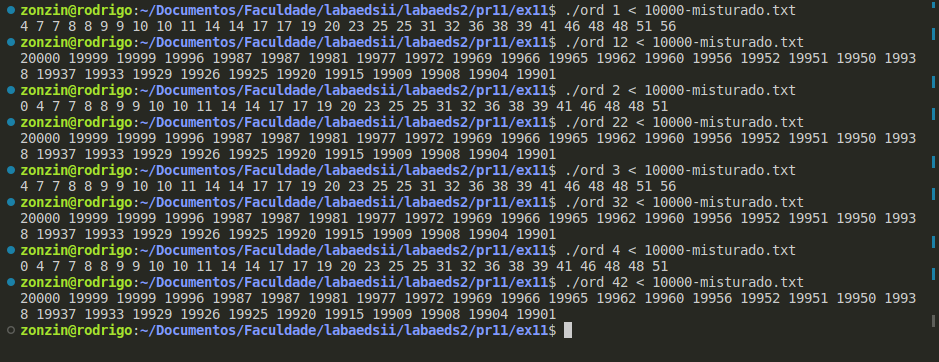
\includegraphics[width=10cm]{imgs/resultadoAlgoritmos.png}

	\caption{Todos os algoritmos}
\end{figure}

\newpage
\section{Tempos}
Usando o script em Python, obtemos os seguintes tempos: 

\begin{figure}[h!]
	\centering
	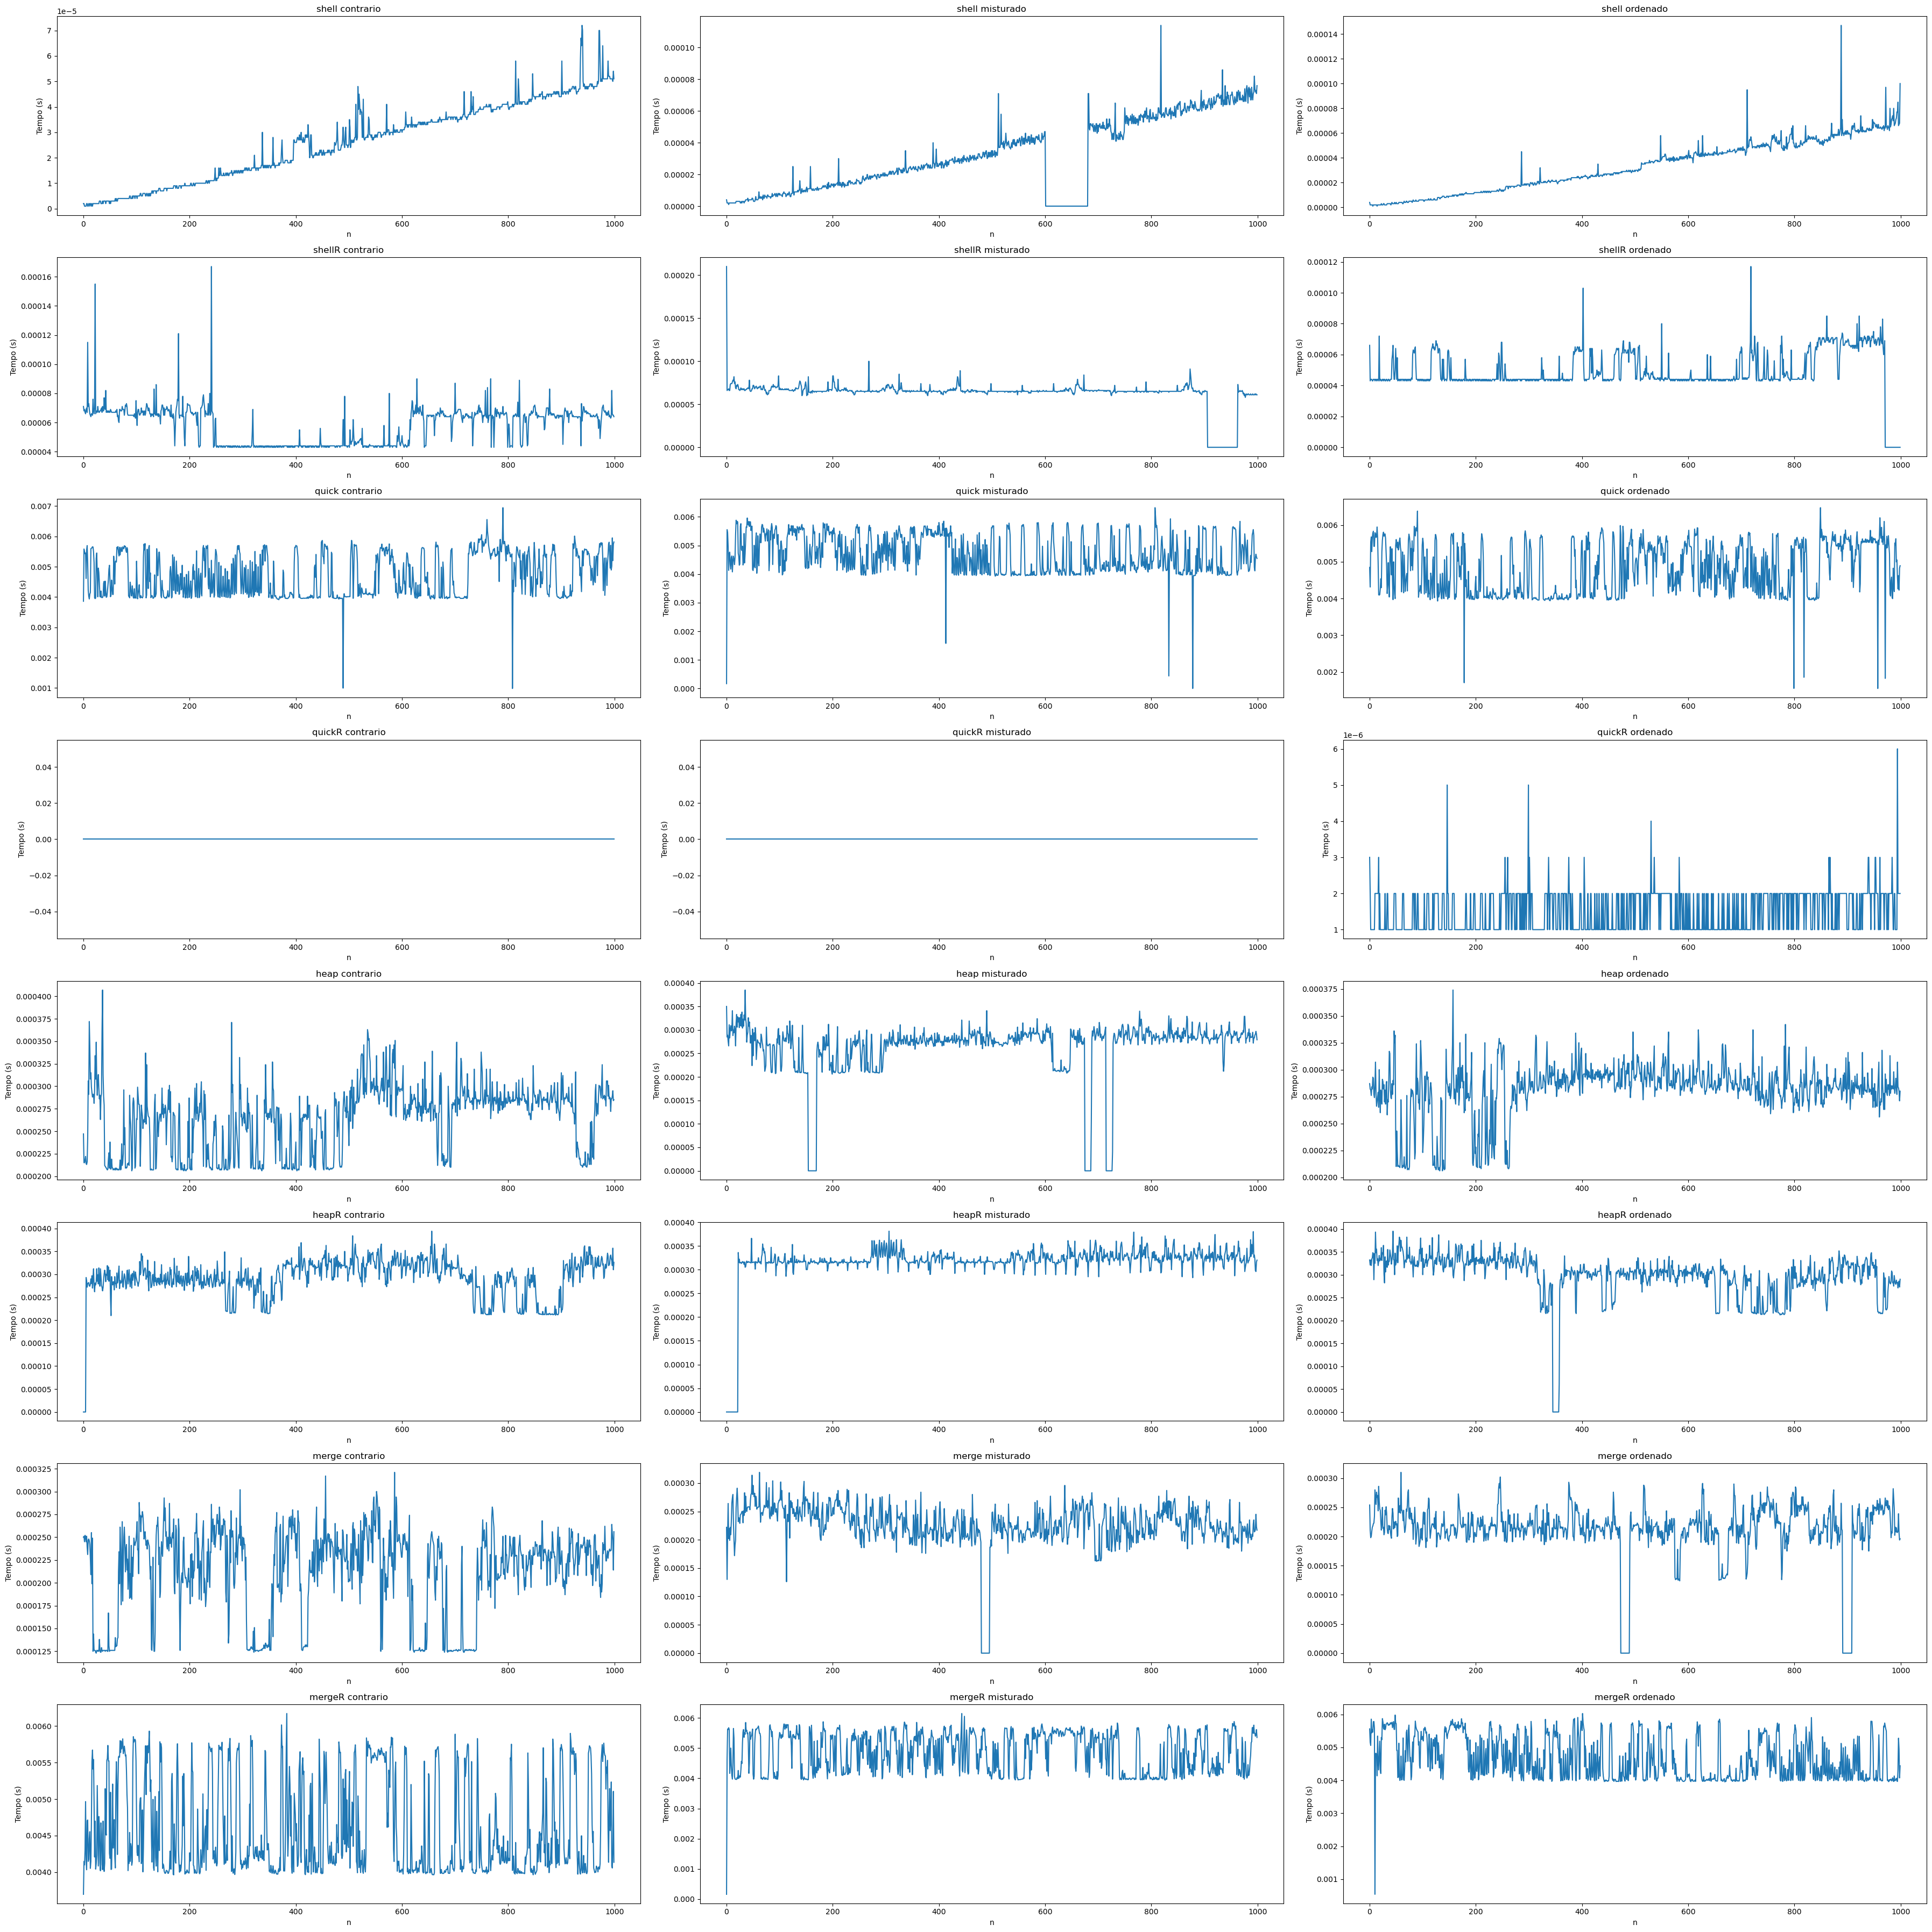
\includegraphics[width=1\linewidth]{imgs/tempo}
	\caption{Algoritmos vs tempo vs $n$}
	\label{fig:tempo}
\end{figure}

\section{Códigos}

\lstinputlisting{../ex11/ordenacao.c}







\newpage


%\bibliographystyle{apalike}
%\bibliographystyle{authordate1}
%\bibliography{referencia.bib}

\end{document}